\section{Removing Vertices}
\label{sect:removing-vertices}

Clusters in the underlying data set can also fade and eventually cease to exist.
In this case, we want to be able to remove existing vertices of the cluster graph.
We make the same distinction here as when inserting vertices: we can remove internal vertices or vertices that lie on the cluster graph's outer face.




\paragraph{Removing Internal Vertices}

When removing an internal vertex of the filtered cluster graph, we must ensure that the graph remains internally triangulated.
This property is preserved iff the internal vertex we want to remove has degree 3.
Removing vertices with a higher degree would create holes in the graph.
If one wants to remove a vertex with degree 4 or higher, one must first change the adjacencies on the inside of the cluster graph using edge flips, discussed in \cref{sect:flipping-edges}.
\Cref{fig:remove-vertex-example-internal} shows an example of a valid removal of an internal vertex.

\begin{figure}[H]
	\centering
	\subfigure[]{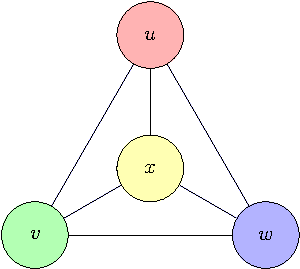
\includegraphics[height=28mm]{Resources/RemoveVertex-Example-Internal-1.pdf}}
	\quad
	\subfigure[]{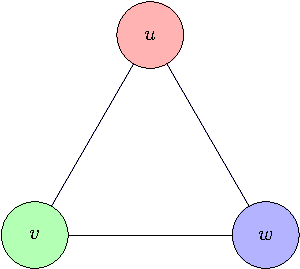
\includegraphics[height=28mm]{Resources/RemoveVertex-Example-Internal-2.pdf}}
	\qquad
	\subfigure[]{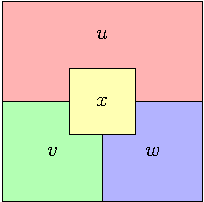
\includegraphics[height=28mm]{Resources/RemoveVertex-Example-Internal-3.pdf}}
	\quad
	\subfigure[]{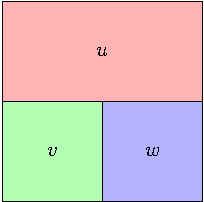
\includegraphics[height=28mm]{Resources/RemoveVertex-Example-Internal-4.pdf}}
	\caption{A cluster graph and a polygonal dual thereof, before (a, c) and after (b, d) removing the internal vertex $x$ with degree 3.}
	\label{fig:remove-vertex-example-internal}
\end{figure}

In order not to create holes in the contact representation, the incident faces must take over the area that the face to be removed used to occupy.
Let $x$ denote the internal vertex we want to remove in the primal and $u$, $v$, and $w$ its three neighbors.
Let $p_{uvx}$ ($p_{vwx}$, $p_{uwx}$) denote the vertex where face $x$ meets faces $u$ and $v$ ($v$ and $w$, $w$ and $u$) in the dual.
\Cref{subfig:remove-vertex-illustration-1} shows how these vertices might look for the example from above.

\begin{figure}[H]
	\centering
	\subfigure[]{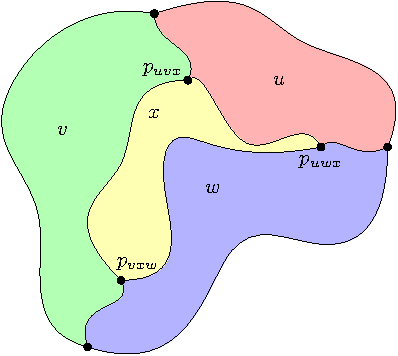
\includegraphics[width=45mm]{Resources/RemoveVertex-Illustration-1.pdf}\label{subfig:remove-vertex-illustration-1}}
	\quad
	\subfigure[]{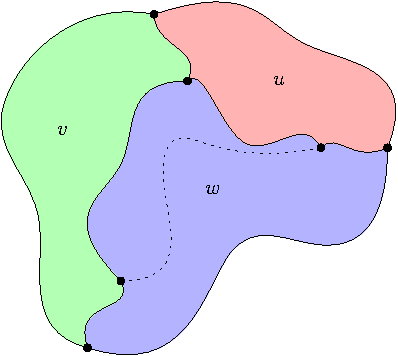
\includegraphics[width=45mm]{Resources/RemoveVertex-Illustration-2.pdf}\label{subfig:remove-vertex-illustration-2}}
	\caption{Removing an internal face $x$ incident to the faces $u$, $v$, and $w$.}
	\label{fig:remove-vertex-illustration}
\end{figure}

To remove the internal face $x$, we simply remove its boundary with one of its neighboring faces.
In doing so, the two faces merge.
In practice, this works well because large clusters do not disappear at a moment's notice, and small clusters generally occupy a minimal area such that the operation is barely noticeable.

With this trivial removal of vertices from the filtered cluster graph, the question arises why we only allow this for vertices of degree 3.
Let us assume we want to remove a face that is adjacent to $n \geq 4$ other faces.
By removing one of the boundaries with its neighboring faces, we would create $n - 3$ new adjacencies that were not there before, as illustrated in \cref{fig:remove-vertex-nondeterministic-adjacencies}.
The respective edges would also need to be inserted into the cluster graph.
Most importantly, though, which new adjacencies would be created depends on which one of the $n$ boundaries is dropped.
Considering future dynamic operations must remain applicable to the cluster graph and the map, we cannot allow such a non-deterministic operation.
Instead, the excess edges need to be flipped away before removing the vertex is allowed, so that the operation remains deterministic.

\begin{figure}[H]
	\centering
	\subfigure[]{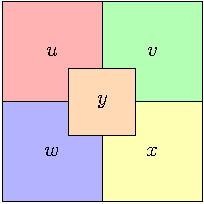
\includegraphics[height=28mm]{Resources/RemoveVertex-NondeterministicAdjacencies-1.pdf}}
	\quad
	\subfigure[]{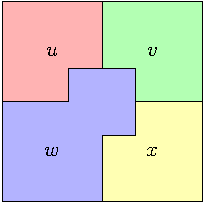
\includegraphics[height=28mm]{Resources/RemoveVertex-NondeterministicAdjacencies-2.pdf}}
	\qquad
	\subfigure[]{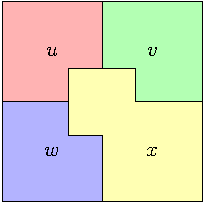
\includegraphics[height=28mm]{Resources/RemoveVertex-NondeterministicAdjacencies-3.pdf}}
	\caption{Non-deterministic removal of an internal face with four neighbors. Removing the $w$-$y$-boundary creates a $w$-$v$-adjacency (b) while removing the $x$-$y$-boundary creates an $x$-$u$-adjacency (c).}
	\label{fig:remove-vertex-nondeterministic-adjacencies}
\end{figure}



\paragraph{Removing External Vertices}

When removing vertices on the outer face of the filtered cluster graph along with its incident edges, we must ensure that the graph remains biconnected afterward.
Similar to inserting vertices on the outer face, we restrict ourselves to removing vertices on the outer face that have degree 2.
If we need to remove a vertex with a higher degree, the additional edges need to be removed first, as discussed in \cref{sect:flipping-edges}.
As a consequence, the operation is only permitted iff the graph has four or more vertices before the vertex' removal.
\Cref{fig:remove-vertex-example-external} shows an example of a valid removal of a vertex on the outer face.

\begin{figure}[H]
	\centering
	\subfigure[]{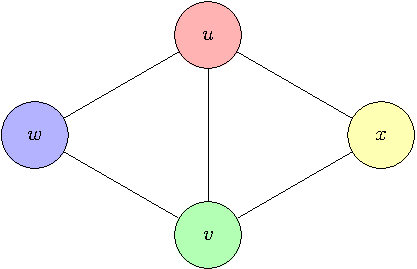
\includegraphics[height=28mm]{Resources/RemoveVertex-Example-External-1.pdf}}
	\quad
	\subfigure[]{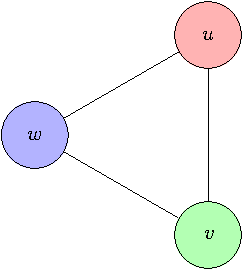
\includegraphics[height=28mm]{Resources/RemoveVertex-Example-External-2.pdf}}
	\qquad
	\subfigure[]{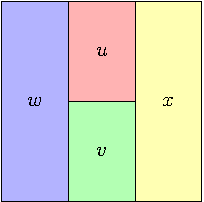
\includegraphics[height=28mm]{Resources/RemoveVertex-Example-External-3.pdf}}
	\quad
	\subfigure[]{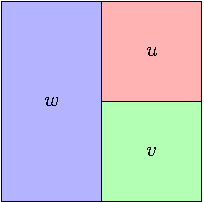
\includegraphics[height=28mm]{Resources/RemoveVertex-Example-External-4.pdf}}
	\caption{A cluster graph and a polygonal dual thereof, before (a, c) and after (b, d) removing the vertex $x$ on the outer face.}
	\label{fig:remove-vertex-example-external}
\end{figure}

This operation, too, is just a special case of the vertex removal discussed above.
Referring to the construction of the augmented dual again, with the helper vertex $v^+$ and edges $\{v^+,\cdot\}$, removable vertices $x$ on the outer face of the cluster graph lie in a triangle formed by its two neighbors $u$ and $v$ and the helper vertex $v^+$.

The construction outlined above translates 1-to-1 to removing vertices from the outer face, except one of the three neighboring faces is the implicit outer face.
In our implementation, we always remove the boundary of $x$ with the outer face and thereby transfer the area to the outer face.
